% Options for packages loaded elsewhere
\PassOptionsToPackage{unicode}{hyperref}
\PassOptionsToPackage{hyphens}{url}
%
\documentclass[
  12pt,
  landscape]{article}
\usepackage{lmodern}
\usepackage{amssymb,amsmath}
\usepackage{ifxetex,ifluatex}
\ifnum 0\ifxetex 1\fi\ifluatex 1\fi=0 % if pdftex
  \usepackage[T1]{fontenc}
  \usepackage[utf8]{inputenc}
  \usepackage{textcomp} % provide euro and other symbols
\else % if luatex or xetex
  \usepackage{unicode-math}
  \defaultfontfeatures{Scale=MatchLowercase}
  \defaultfontfeatures[\rmfamily]{Ligatures=TeX,Scale=1}
\fi
% Use upquote if available, for straight quotes in verbatim environments
\IfFileExists{upquote.sty}{\usepackage{upquote}}{}
\IfFileExists{microtype.sty}{% use microtype if available
  \usepackage[]{microtype}
  \UseMicrotypeSet[protrusion]{basicmath} % disable protrusion for tt fonts
}{}
\makeatletter
\@ifundefined{KOMAClassName}{% if non-KOMA class
  \IfFileExists{parskip.sty}{%
    \usepackage{parskip}
  }{% else
    \setlength{\parindent}{0pt}
    \setlength{\parskip}{6pt plus 2pt minus 1pt}}
}{% if KOMA class
  \KOMAoptions{parskip=half}}
\makeatother
\usepackage{xcolor}
\IfFileExists{xurl.sty}{\usepackage{xurl}}{} % add URL line breaks if available
\IfFileExists{bookmark.sty}{\usepackage{bookmark}}{\usepackage{hyperref}}
\hypersetup{
  pdftitle={ECON 21110 - Applied Microeconometrics - Assignment 2},
  pdfauthor={Jack Ogle},
  hidelinks,
  pdfcreator={LaTeX via pandoc}}
\urlstyle{same} % disable monospaced font for URLs
\usepackage[margin=1in]{geometry}
\usepackage{color}
\usepackage{fancyvrb}
\newcommand{\VerbBar}{|}
\newcommand{\VERB}{\Verb[commandchars=\\\{\}]}
\DefineVerbatimEnvironment{Highlighting}{Verbatim}{commandchars=\\\{\}}
% Add ',fontsize=\small' for more characters per line
\usepackage{framed}
\definecolor{shadecolor}{RGB}{248,248,248}
\newenvironment{Shaded}{\begin{snugshade}}{\end{snugshade}}
\newcommand{\AlertTok}[1]{\textcolor[rgb]{0.94,0.16,0.16}{#1}}
\newcommand{\AnnotationTok}[1]{\textcolor[rgb]{0.56,0.35,0.01}{\textbf{\textit{#1}}}}
\newcommand{\AttributeTok}[1]{\textcolor[rgb]{0.77,0.63,0.00}{#1}}
\newcommand{\BaseNTok}[1]{\textcolor[rgb]{0.00,0.00,0.81}{#1}}
\newcommand{\BuiltInTok}[1]{#1}
\newcommand{\CharTok}[1]{\textcolor[rgb]{0.31,0.60,0.02}{#1}}
\newcommand{\CommentTok}[1]{\textcolor[rgb]{0.56,0.35,0.01}{\textit{#1}}}
\newcommand{\CommentVarTok}[1]{\textcolor[rgb]{0.56,0.35,0.01}{\textbf{\textit{#1}}}}
\newcommand{\ConstantTok}[1]{\textcolor[rgb]{0.00,0.00,0.00}{#1}}
\newcommand{\ControlFlowTok}[1]{\textcolor[rgb]{0.13,0.29,0.53}{\textbf{#1}}}
\newcommand{\DataTypeTok}[1]{\textcolor[rgb]{0.13,0.29,0.53}{#1}}
\newcommand{\DecValTok}[1]{\textcolor[rgb]{0.00,0.00,0.81}{#1}}
\newcommand{\DocumentationTok}[1]{\textcolor[rgb]{0.56,0.35,0.01}{\textbf{\textit{#1}}}}
\newcommand{\ErrorTok}[1]{\textcolor[rgb]{0.64,0.00,0.00}{\textbf{#1}}}
\newcommand{\ExtensionTok}[1]{#1}
\newcommand{\FloatTok}[1]{\textcolor[rgb]{0.00,0.00,0.81}{#1}}
\newcommand{\FunctionTok}[1]{\textcolor[rgb]{0.00,0.00,0.00}{#1}}
\newcommand{\ImportTok}[1]{#1}
\newcommand{\InformationTok}[1]{\textcolor[rgb]{0.56,0.35,0.01}{\textbf{\textit{#1}}}}
\newcommand{\KeywordTok}[1]{\textcolor[rgb]{0.13,0.29,0.53}{\textbf{#1}}}
\newcommand{\NormalTok}[1]{#1}
\newcommand{\OperatorTok}[1]{\textcolor[rgb]{0.81,0.36,0.00}{\textbf{#1}}}
\newcommand{\OtherTok}[1]{\textcolor[rgb]{0.56,0.35,0.01}{#1}}
\newcommand{\PreprocessorTok}[1]{\textcolor[rgb]{0.56,0.35,0.01}{\textit{#1}}}
\newcommand{\RegionMarkerTok}[1]{#1}
\newcommand{\SpecialCharTok}[1]{\textcolor[rgb]{0.00,0.00,0.00}{#1}}
\newcommand{\SpecialStringTok}[1]{\textcolor[rgb]{0.31,0.60,0.02}{#1}}
\newcommand{\StringTok}[1]{\textcolor[rgb]{0.31,0.60,0.02}{#1}}
\newcommand{\VariableTok}[1]{\textcolor[rgb]{0.00,0.00,0.00}{#1}}
\newcommand{\VerbatimStringTok}[1]{\textcolor[rgb]{0.31,0.60,0.02}{#1}}
\newcommand{\WarningTok}[1]{\textcolor[rgb]{0.56,0.35,0.01}{\textbf{\textit{#1}}}}
\usepackage{graphicx,grffile}
\makeatletter
\def\maxwidth{\ifdim\Gin@nat@width>\linewidth\linewidth\else\Gin@nat@width\fi}
\def\maxheight{\ifdim\Gin@nat@height>\textheight\textheight\else\Gin@nat@height\fi}
\makeatother
% Scale images if necessary, so that they will not overflow the page
% margins by default, and it is still possible to overwrite the defaults
% using explicit options in \includegraphics[width, height, ...]{}
\setkeys{Gin}{width=\maxwidth,height=\maxheight,keepaspectratio}
% Set default figure placement to htbp
\makeatletter
\def\fps@figure{htbp}
\makeatother
\setlength{\emergencystretch}{3em} % prevent overfull lines
\providecommand{\tightlist}{%
  \setlength{\itemsep}{0pt}\setlength{\parskip}{0pt}}
\setcounter{secnumdepth}{-\maxdimen} % remove section numbering
\usepackage{dcolumn}
\usepackage{float}

\title{ECON 21110 - Applied Microeconometrics - Assignment 2}
\author{Jack Ogle}
\date{}

\begin{document}
\maketitle

Problem 1

\begin{enumerate}
\def\labelenumi{(\alph{enumi})}
\item
\end{enumerate}

\begin{table}[H] \centering 
  \caption{Regression Results (a)} 
  \label{} 
\begin{tabular}{@{\extracolsep{5pt}}lc} 
\\[-1.8ex]\hline 
\hline \\[-1.8ex] 
 & \multicolumn{1}{c}{\textit{Dependent variable:}} \\ 
\cline{2-2} 
\\[-1.8ex] & colgpa \\ 
\hline \\[-1.8ex] 
 female & 0.142$^{***}$ \\ 
  & (0.020) \\ 
  & \\ 
 Constant & 2.589$^{***}$ \\ 
  & (0.014) \\ 
  & \\ 
\hline \\[-1.8ex] 
Observations & 4,137 \\ 
R$^{2}$ & 0.012 \\ 
Adjusted R$^{2}$ & 0.011 \\ 
Residual Std. Error & 0.655 (df = 4135) \\ 
F Statistic & 48.157$^{***}$ (df = 1; 4135) \\ 
\hline 
\hline \\[-1.8ex] 
\textit{Note:}  & \multicolumn{1}{r}{$^{*}$p$<$0.1; $^{**}$p$<$0.05; $^{***}$p$<$0.01} \\ 
 & \multicolumn{1}{r}{Standard errors in parentheses} \\ 
\end{tabular} 
\end{table}

The female coefficient is difference in the average of college gpa
between females and males. On average a female's gpa is 0.142 higher
than a male's.

\begin{enumerate}
\def\labelenumi{(\alph{enumi})}
\setcounter{enumi}{1}
\item
\end{enumerate}

\begin{verbatim}
## `stat_bin()` using `bins = 30`. Pick better value with `binwidth`.
\end{verbatim}

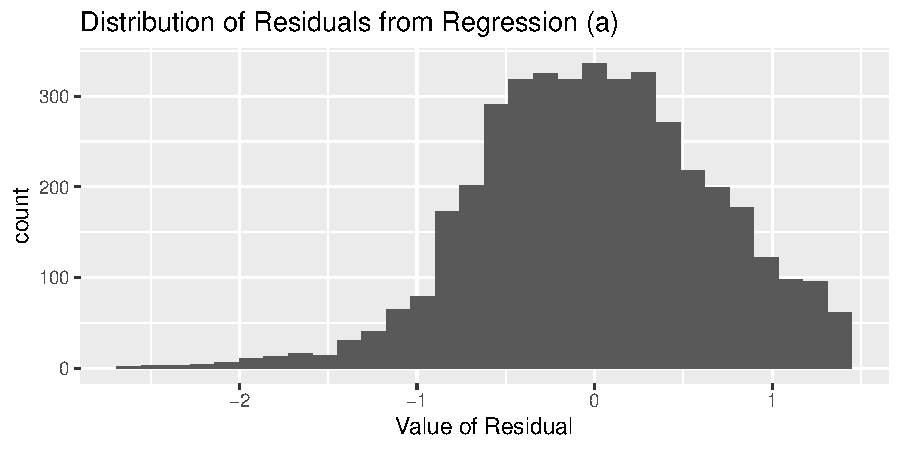
\includegraphics{Ogle_MicroMetricsAssignment_2_Q1_files/figure-latex/unnamed-chunk-3-1.pdf}

\begin{verbatim}
## 
##  Shapiro-Wilk normality test
## 
## data:  modelA$residuals
## W = 0.99245, p-value = 5.352e-14
\end{verbatim}

In the figure above we can see a histogram of the residuals. The
regression looks normal but we must do a test statistic to know for
sure. We will use the shapiro-wilk test for normality. We get the result
W = 0.99245, p-value = 5.352e-14. This suggest that the distribution is
not normal and that we can reject the null hypothesis of
homoskedasticity. The model is heteroskedastic.

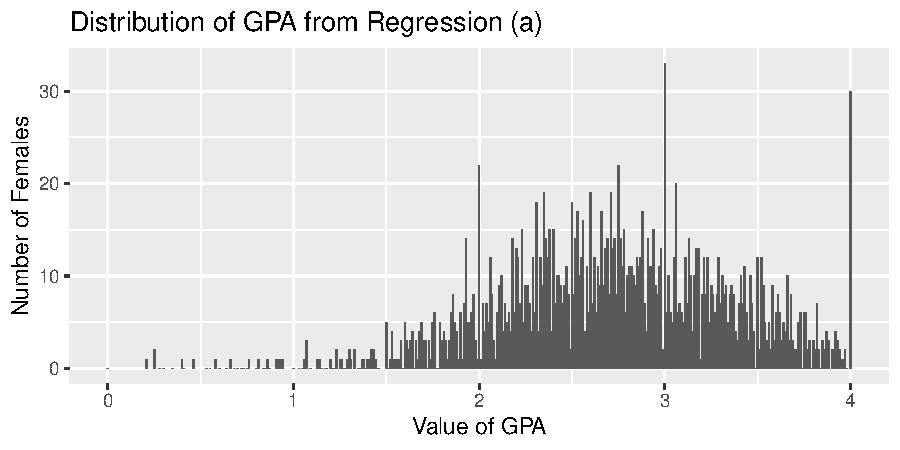
\includegraphics{Ogle_MicroMetricsAssignment_2_Q1_files/figure-latex/unnamed-chunk-4-1.pdf}

\begin{enumerate}
\def\labelenumi{(\alph{enumi})}
\setcounter{enumi}{2}
\tightlist
\item
  We first want to standardize our sat scores by subtracting each
  observation by the mean and dividing by the standard deviation. We
  standardize sat scores to reduce multicollinearity among the
  independent variables. This makes the sat score more meaningful
  because the interpretation of sat coefficient one standard
  deviation.\\
  \[
  colgpa_i = \hat{\beta_0} + \hat{\beta_1}female_i + \hat{\beta_2}standardSat_i+ U_i
  \]
\end{enumerate}

\begin{table}[!htbp] \centering 
  \caption{Regression Results (c)} 
  \label{} 
\begin{tabular}{@{\extracolsep{5pt}}lc} 
\\[-1.8ex]\hline 
\hline \\[-1.8ex] 
 & \multicolumn{1}{c}{\textit{Dependent variable:}} \\ 
\cline{2-2} 
\\[-1.8ex] & colgpa \\ 
\hline \\[-1.8ex] 
 female & 0.231$^{***}$ \\ 
  & (0.019) \\ 
  & \\ 
 standardSat & 0.287$^{***}$ \\ 
  & (0.009) \\ 
  & \\ 
 Constant & 2.549$^{***}$ \\ 
  & (0.012) \\ 
  & \\ 
\hline \\[-1.8ex] 
Observations & 4,137 \\ 
R$^{2}$ & 0.197 \\ 
Adjusted R$^{2}$ & 0.196 \\ 
Residual Std. Error & 0.590 (df = 4134) \\ 
F Statistic & 506.099$^{***}$ (df = 2; 4134) \\ 
\hline 
\hline \\[-1.8ex] 
\textit{Note:}  & \multicolumn{1}{r}{$^{*}$p$<$0.1; $^{**}$p$<$0.05; $^{***}$p$<$0.01} \\ 
 & \multicolumn{1}{r}{Standard errors in parentheses} \\ 
\end{tabular} 
\end{table}

There is an increase in the coefficient from 0.142 to 0.287 when we add
in SAT scores as an independent variable.

\[
\tilde{\beta_1} = \hat{\beta_1} + \hat{\beta_2}\tilde{\delta_1}
\] Where \(\tilde{\beta_1}\) is the estimate from SLR and
\(\hat{\beta_1}\) and \(\hat{\beta_2}\) are the estimates from MLR.
\(\tilde{\delta_1}\) is the coefficient estimate from the following
regression. \[
standardSat_i = \tilde{\delta_0} + \tilde{\delta_1}female_i + U_i
\]

We can see that \(\tilde{\delta_1}\) has a negative sign implying that
sat and female are negatively correlated. We know this by knowing that
\(\hat{\beta_1}\), \(\tilde{\beta_1}\) and \(\hat{\beta_2}\) are
positive. If all the estimators are positive using the equation above we
know that \(\tilde{\delta_1}\) has a negative sign.

\begin{table}[!htbp] \centering 
  \caption{Regression Results (c)} 
  \label{} 
\begin{tabular}{@{\extracolsep{5pt}}lc} 
\\[-1.8ex]\hline 
\hline \\[-1.8ex] 
 & \multicolumn{1}{c}{\textit{Dependent variable:}} \\ 
\cline{2-2} 
\\[-1.8ex] & standardSat \\ 
\hline \\[-1.8ex] 
 female & $-$0.309$^{***}$ \\ 
  & (0.031) \\ 
  & \\ 
 Constant & 0.139$^{***}$ \\ 
  & (0.021) \\ 
  & \\ 
\hline \\[-1.8ex] 
Observations & 4,137 \\ 
R$^{2}$ & 0.024 \\ 
Adjusted R$^{2}$ & 0.023 \\ 
Residual Std. Error & 0.988 (df = 4135) \\ 
F Statistic & 100.082$^{***}$ (df = 1; 4135) \\ 
\hline 
\hline \\[-1.8ex] 
\textit{Note:}  & \multicolumn{1}{r}{$^{*}$p$<$0.1; $^{**}$p$<$0.05; $^{***}$p$<$0.01} \\ 
 & \multicolumn{1}{r}{Standard errors in parentheses} \\ 
\end{tabular} 
\end{table}

We get that the female coefficient is -0.309 implying that on average
being a female results in a SAT score 30.9\% lower than being a male.

Because female and sat are negatively correlated, when sat is added into
the regression our coefficient increases from 0.142 to 0.231 meaning
that there was a negative OVB in the first model. We calculate the
negative bias by subtracting the coefficient for female without sat and
the coefficient for female with sat. 0.142-0.231 = -0.089.

\begin{enumerate}
\def\labelenumi{(\alph{enumi})}
\setcounter{enumi}{3}
\item
\end{enumerate}

We estimate our model with OLS: \[
colgpa_i = \hat{\beta_0} + \hat{\beta_1}female_i + \hat{\beta_2}sat_i+ U_i
\] See table 2 for results of that regression. From that regression we
obtain the residuals \(\hat{U}\).

Then we regress the squared residuals \(\hat{U^2}\) on female and sat.
From that we obtain an R-squared value \(R^2_{\hat{U^2}}\) of 0.00261.

We then use the following formula to compute our F-Statistic: \[
F = \frac{R^2_{\hat{U^2}}/k}{(1-R^2_{\hat{U^2}})/(n-k-1)}
\] We calculate a chi squared test using the chi value and the degrees
of freedom. Which gives us the following values.

F-statistic = 5.409 p-value = 0.00451

Since the p-value is less than 0.05, we can reject the null hypothesis
of homoskedasticity. There for heteroskedasticity is present.

For the White test, we must regress our residuals squared over all the
independent variables, the squares of the independent variables, and the
cross-products between the independent variables. From that regression
we see an p-value with a value of 0.0085. Because this p-value is less
than 0.05 we reject our null hypothesis of homoskedasticity.

\begin{enumerate}
\def\labelenumi{(\alph{enumi})}
\setcounter{enumi}{4}
\item
\end{enumerate}

\begin{table}[H] \centering 
  \caption{Regression Results (c)} 
  \label{} 
\begin{tabular}{@{\extracolsep{5pt}}lcc} 
\\[-1.8ex]\hline 
\hline \\[-1.8ex] 
 & \multicolumn{2}{c}{\textit{Dependent variable:}} \\ 
\cline{2-3} 
\\[-1.8ex] & \multicolumn{2}{c}{colgpa} \\ 
 & Non-Robust Std. Errors & Robust Std. Errors \\ 
\\[-1.8ex] & (1) & (2)\\ 
\hline \\[-1.8ex] 
 female & 0.231$^{***}$ & 0.231$^{***}$ \\ 
  & (0.019) & (0.018) \\ 
  & & \\ 
 standardSat & 0.287$^{***}$ & 0.287$^{***}$ \\ 
  & (0.009) & (0.009) \\ 
  & & \\ 
 Constant & 2.549$^{***}$ & 2.549$^{***}$ \\ 
  & (0.012) & (0.013) \\ 
  & & \\ 
\hline \\[-1.8ex] 
Observations & 4,137 & 4,137 \\ 
R$^{2}$ & 0.197 & 0.197 \\ 
Adjusted R$^{2}$ & 0.196 & 0.196 \\ 
Residual Std. Error (df = 4134) & 0.590 & 0.590 \\ 
F Statistic (df = 2; 4134) & 506.099$^{***}$ & 536.1$^{***}$ \\ 
\hline 
\hline \\[-1.8ex] 
\textit{Note:}  & \multicolumn{2}{r}{$^{*}$p$<$0.1; $^{**}$p$<$0.05; $^{***}$p$<$0.01} \\ 
 & \multicolumn{2}{r}{Standard errors in parentheses} \\ 
\end{tabular} 
\end{table}

Observing table 4 we see that for the female coefficient the robust
standard error is less than the non-robust standard error. For the sat
coefficient we see that the robust and non-robust standard error are the
same. And for the constant we get that the robust standard error is
slightly larger than the non-robust standard error.

Additionally, our F-statistic increases from 506.099 to 536.19.

These new results support our findings from c.~Because the assumption of
homoskedasticity the null hypothesis was rejected, there is variance
among our residuals as we change our independent variables. The model is
heteroskedastic we would employ robust standard errors to correct for
the higher variance in among residuals the model as the independent
variables change.

\begin{enumerate}
\def\labelenumi{(\alph{enumi})}
\setcounter{enumi}{5}
\tightlist
\item
  We estimate the following \[
  colgpa = \beta_0 + \beta_1sat + \beta_2female + \beta_3sat^2
  \]
\end{enumerate}

\begin{table}[H] \centering 
  \caption{Regression Results (f)} 
  \label{} 
\begin{tabular}{@{\extracolsep{5pt}}lc} 
\\[-1.8ex]\hline 
\hline \\[-1.8ex] 
 & \multicolumn{1}{c}{\textit{Dependent variable:}} \\ 
\cline{2-2} 
\\[-1.8ex] & colgpa \\ 
\hline \\[-1.8ex] 
 sat & 0.285$^{***}$ \\ 
  & (0.009) \\ 
  & \\ 
 female & 0.239$^{***}$ \\ 
  & (0.019) \\ 
  & \\ 
 sat$^{2}$ & 0.038$^{***}$ \\ 
  & (0.006) \\ 
  & \\ 
 Constant & 2.507$^{***}$ \\ 
  & (0.014) \\ 
  & \\ 
\hline \\[-1.8ex] 
Observations & 4,137 \\ 
R$^{2}$ & 0.204 \\ 
Adjusted R$^{2}$ & 0.203 \\ 
Residual Std. Error & 0.588 (df = 4133) \\ 
F Statistic & 352.873$^{***}$ (df = 3; 4133) \\ 
\hline 
\hline \\[-1.8ex] 
\textit{Note:}  & \multicolumn{1}{r}{$^{*}$p$<$0.1; $^{**}$p$<$0.05; $^{***}$p$<$0.01} \\ 
 & \multicolumn{1}{r}{Standard errors in parentheses} \\ 
\end{tabular} 
\end{table}

With this regression result the functional relationship between colgpa
and sat is likely linear. We can reject a non-linear relationship. We
fail to reject \({H_0: \beta_3 = 0}\). This suggests that there is a
linear relationship between colgpa and sat.

The coefficient estimator for sat scores on college gpa is that for
every increase in a standard deviation of SAT score there is a 0.287
increase in College GPA. This is pretty low this can be explained by a
the fact that we have a non random sample. Colleges choose the students
they admit based on various factors including SAT scores. Not all
students who took the SAT when to college, so we are missing a part of
our random sample. It is likely that those students who did not go to
college have lower SAT scores than those who did. Therefore sat scores
should have a higher impact on college gpa but because we need to
include everyone in the random sample who took the SAT it is smaller.

\begin{enumerate}
\def\labelenumi{(\alph{enumi})}
\setcounter{enumi}{6}
\item
  MLR.4 is the Zero Conditional Mean Assumption which states none of the
  independent variables are correlated to any variables in the error
  term. I think that the Zero Conditional Mean assumption does not hold
  because there are variables in the error term that are correlated with
  independent variables. For example, household income is correlated
  with sat scores. If we included metrics like parental income,
  household income. and IQ it would be more credible. It would be more
  credible because fewer variables in the error term would be correlated
  with independent variables.
\item
  An ideal randomized experiment would be to clone one man and one women
  who take the same courses, have the same ability and socio-economic
  background. We should also attempt to study students from the same
  college. We want to compare students with the same major and who take
  the same classes. We should also compare students with similar IQ and
  ability to study, think, and learn. Essentially, we would like to
  control for every variable that might lead to a violation of the Zero
  Conditional Mean assumption. If we can satisfy the Zero Conditional
  Mean Assumption than we can understand the causal effect of female on
  college gpa without any confounding variables. This is because if the
  zero conditional mean is satisfied than the error term does not show
  any systematic pattern and have a mean of zero regardless of the
  independent variables that we choose.
\item
  If we attempted to implement the ideal randomized experiment we would
  run into some challenges. It is not possible to control for every
  confounding variable. It is impossible to find a male clone for every
  female. However, if we are not able to find perfect clones with the
  same ability and socio-economic background. We might be able to find
  matches for ability measures like IQ and KWW. We might also be able to
  control for the different majors of study. We also would be able to
  control for socio-economic background by controlling for parental
  income and household income.
\end{enumerate}

Problem 2

\begin{enumerate}
\def\labelenumi{(\alph{enumi})}
\tightlist
\item
  We estimate the population model: \[
  price_i = \beta_0 + \beta_1sqrft_i + \beta_2bdrms_i + \beta_3lotsize_i + U_i
  \]
\end{enumerate}

\begin{table}[!htbp] \centering 
  \caption{Regression Results (a)} 
  \label{} 
\begin{tabular}{@{\extracolsep{5pt}}lc} 
\\[-1.8ex]\hline 
\hline \\[-1.8ex] 
 & \multicolumn{1}{c}{\textit{Dependent variable:}} \\ 
\cline{2-2} 
\\[-1.8ex] & price \\ 
\hline \\[-1.8ex] 
 sqrft & 0.123 \\ 
  & (0.013)$^{***}$ \\ 
  & t = 9.275$^{***}$ \\ 
  & \\ 
 bdrms & 13.853 \\ 
  & (9.010) \\ 
  & t = 1.537 \\ 
  & \\ 
 lotsize & 0.002 \\ 
  & (0.001)$^{***}$ \\ 
  & t = 3.220$^{***}$ \\ 
  & \\ 
 Constant & $-$21.770 \\ 
  & (29.475) \\ 
  & t = $-$0.739 \\ 
  & \\ 
\hline \\[-1.8ex] 
Observations & 88 \\ 
R$^{2}$ & 0.672 \\ 
Adjusted R$^{2}$ & 0.661 \\ 
Residual Std. Error & 59.833 (df = 84) \\ 
F Statistic & 57.460$^{***}$ (df = 3; 84) \\ 
\hline 
\hline \\[-1.8ex] 
\textit{Note:}  & \multicolumn{1}{r}{$^{*}$p$<$0.1; $^{**}$p$<$0.05; $^{***}$p$<$0.01} \\ 
 & \multicolumn{1}{r}{Standard errors in parentheses. T-Statistics below standard errors} \\ 
\end{tabular} 
\end{table}

According to our regression results from Table 1 we can interpret the
following. All other independent variables constant for every increase
in square foot there is an price that is increased by 123 dollars on
average.

All other independent variables constant for every unit increase in lot
size there is an 2 dollar increase in price on average.

All other independent variables constant for every unit increase in
bedrooms there is an 13,853 dollar increase in price on average. This
values is not statistically significant in this regression because the p
value is greater than 0.05.

There is no logical interpretation for the constant as the price of a
house cannot be negative.

\begin{enumerate}
\def\labelenumi{(\alph{enumi})}
\setcounter{enumi}{1}
\item
  The OLS estimate for the parameters in the model we estimated in (a)
  is biased. This is because it violated MLR.4 (the Zero Conditional
  Mean Assumption). There are variables in the error term that are
  correlated with independent variables. For example, variables that
  measure the location of the house is likely correlated with all three
  of the independent variables. If the location is a densely populated
  urban area then it will likely have less square footage, bedrooms, and
  a smaller lot size. Other variables related to the location of the
  house like property tax and average income of the zip-code are also in
  the error term and correlated with the independent variables.
\item
  If we could collect additional data on environmental factors, I would
  include the variables that measure the location of the house. These
  variables include proximity to a large urban area, property tax,
  proximity to a coast, population of the city or town that the house is
  in. I would want to control for all the variables related to location
  of the house because these are correlated with the independent size
  variables and the price. The most important omitted variable that
  would affect the OLS estimator would be property tax the town that the
  house is located in. This would reduced our OVB and make MLR.4 more
  credible. This is because property tax can tell us a lot about the
  location of house. It can tell us if the house is in a wealthy area or
  poor area. If it is in a high crime or low crime area. When we add
  this independent into our regression we can control for crime,
  relative wealth, quality of schools in the area. And when we control
  for these variables we make MLR.4 more credible.
\item
\end{enumerate}

\begin{enumerate}
\def\labelenumi{\roman{enumi})}
\tightlist
\item
  We estimate the population model: \[
  price_i = \beta_0 + \beta_1sqrft_i + \beta_2bdrms_i + \beta_3lotsize_i + \beta_4colonial_i + U_i
  \]

  \begin{table}[!htbp] \centering 
    \caption{Regression Results (d-1)} 
    \label{} 
  \begin{tabular}{@{\extracolsep{5pt}}lc} 
  \\[-1.8ex]\hline 
  \hline \\[-1.8ex] 
   & \multicolumn{1}{c}{\textit{Dependent variable:}} \\ 
  \cline{2-2} 
  \\[-1.8ex] & price \\ 
  \hline \\[-1.8ex] 
   sqrft & 0.124 \\ 
    & (0.013)$^{***}$ \\ 
    & t = 9.314$^{***}$ \\ 
    & \\ 
   bdrms & 11.004 \\ 
    & (9.515) \\ 
    & t = 1.156 \\ 
    & \\ 
   lotsize & 0.002 \\ 
    & (0.001)$^{***}$ \\ 
    & t = 3.230$^{***}$ \\ 
    & \\ 
   colonial & 13.716 \\ 
    & (14.637) \\ 
    & t = 0.937 \\ 
    & \\ 
   Constant & $-$24.127 \\ 
    & (29.603) \\ 
    & t = $-$0.815 \\ 
    & \\ 
  \hline \\[-1.8ex] 
  Observations & 88 \\ 
  R$^{2}$ & 0.676 \\ 
  Adjusted R$^{2}$ & 0.660 \\ 
  Residual Std. Error & 59.877 (df = 83) \\ 
  F Statistic & 43.252$^{***}$ (df = 4; 83) \\ 
  \hline 
  \hline \\[-1.8ex] 
  \textit{Note:}  & \multicolumn{1}{r}{$^{*}$p$<$0.1; $^{**}$p$<$0.05; $^{***}$p$<$0.01} \\ 
   & \multicolumn{1}{r}{Standard errors in parentheses. T-Statistics below standard errors} \\ 
  \end{tabular} 
  \end{table}
\item
  According to our regression results from the table above we can
  interpret the following. All other independent variables constant for
  every increase in square foot there is an price that is increased by
  124 dollars on average.
\end{enumerate}

All other independent variables constant for every unit increase in lot
size there is an 2 dollar increase in price on average.

All other independent variables constant for every unit increase in
bedrooms there is an 11,004 dollar increase in price on average. This
values is not statistically significant in this regression because the p
value is greater than 0.05.

All other independent variables constant if the house is a colonial
style there is an 13,716 dollar increase in price compared to non
colonial style houses on average. This values is not statistically
significant in this regression because the p value is greater than 0.05.

When there are no effects from any independent variables, when they are
all equal to zero the average price is -24,127. However, this value is
not statistically significant in this regression because the p value is
greater than 0.05. Additionally this value has no meaning because the
price of the house cannot be negative.

\begin{enumerate}
\def\labelenumi{\roman{enumi})}
\setcounter{enumi}{2}
\tightlist
\item
  \({H_0: \beta_4 = \beta_1 =\beta_2 = \beta_3 }\)
\end{enumerate}

We reject this null hypothesis. Adding the colonial binary variable
reduces the effect of bedrooms on price. However, the effect of square
feet and lot size remain constant with the addition. Adding colonial
into our regression has very little effect on the price. This makes
sense because colonial houses are just a style of house and other
factors that are related to the environment or location would have a
larger impact on price.

\begin{enumerate}
\def\labelenumi{(\alph{enumi})}
\setcounter{enumi}{4}
\item
\end{enumerate}

\begin{enumerate}
\def\labelenumi{\roman{enumi})}
\tightlist
\item
  We estimate the population model: \[
  price_i = \beta_0 + \beta_1sqrft_i + \beta_2bdrms_i + \beta_3lotsize_i + \beta_4colonial_i + U_i
  \]
\item
  According to our regression results from Table 1 we can interpret the
  following. All other independent variables constant for every increase
  in square foot there is an price that is increased by 124 dollars on
  average.
\end{enumerate}

All other independent variables constant for every unit increase in lot
size there is an 2 dollar increase in price on average.

All other independent variables constant for every unit increase in
bedrooms there is an 11,004 dollar increase in price on average. This
values is not statistically significant in this regression because the p
value is greater than 0.05.

All other independent variables constant if the house is a colonial
style there is an 13,716 dollar increase in price compared to non
colonial style houses on average. This values is not statistically
significant in this regression because the p value is greater than 0.05.

When there are no effects from any independent variables, when they are
all equal to zero the average price is -24,127. However, this value is
not statistically significant in this regression because the p value is
greater than 0.05.

To find the OVB we need to subtract all coefficients from the original
regression without colonial (\(\hat\beta_1\)) from the coefficients from
the new regression with colonial (\(\tilde\beta_1\)).

OVB for each independent variable: \[
\hat\beta_1- \tilde\beta_1 =  0.123 - 0.124 = -0.001
\] \[
\hat\beta_2- \tilde\beta_2 = 13.853 - 11.004 = 2.849 \\
\] \[
\hat\beta_3- \tilde\beta_3 = 0.002 -0.002 = 0\\
\] I did not understand whether this question was referring to OVB in
the model or just for each coefficient so I assumed that it was for each
coefficient.

\begin{enumerate}
\def\labelenumi{(\alph{enumi})}
\setcounter{enumi}{5}
\item
\end{enumerate}

\begin{enumerate}
\def\labelenumi{\roman{enumi})}
\tightlist
\item
  We estimate the population model: \[
  price_i = \beta_0 + \beta_1sqrft_i + \beta_2bdrms_i + \beta_3lotsize_i +\beta_4colonial_i + \beta_5sqrft_icolonial_i + \beta_6bdrms_icolonial_i + \beta_7lotsize_icolonial_i + U_i
  \]
\end{enumerate}

\begin{table}[H] \centering 
  \caption{Regression Results (f-1)} 
  \label{} 
\begin{tabular}{@{\extracolsep{5pt}}lc} 
\\[-1.8ex]\hline 
\hline \\[-1.8ex] 
 & \multicolumn{1}{c}{\textit{Dependent variable:}} \\ 
\cline{2-2} 
\\[-1.8ex] & price \\ 
\hline \\[-1.8ex] 
 sqrft & 0.090$^{***}$ \\ 
  & (0.024) \\ 
  & \\ 
 bdrms & 11.225 \\ 
  & (20.369) \\ 
  & \\ 
 lotsize & 0.007$^{***}$ \\ 
  & (0.002) \\ 
  & \\ 
 colonial & $-$30.601 \\ 
  & (62.734) \\ 
  & \\ 
 sqrft:colonial & 0.044 \\ 
  & (0.029) \\ 
  & \\ 
 bdrms:colonial & 1.644 \\ 
  & (22.833) \\ 
  & \\ 
 lotsize:colonial & $-$0.006$^{***}$ \\ 
  & (0.002) \\ 
  & \\ 
 Constant & $-$2.874 \\ 
  & (50.810) \\ 
  & \\ 
\hline \\[-1.8ex] 
Observations & 88 \\ 
R$^{2}$ & 0.709 \\ 
Adjusted R$^{2}$ & 0.684 \\ 
Residual Std. Error & 57.758 (df = 80) \\ 
F Statistic & 27.877$^{***}$ (df = 7; 80) \\ 
\hline 
\hline \\[-1.8ex] 
\textit{Note:}  & \multicolumn{1}{r}{$^{*}$p$<$0.1; $^{**}$p$<$0.05; $^{***}$p$<$0.01} \\ 
 & \multicolumn{1}{r}{Standard errors in parentheses} \\ 
\end{tabular} 
\end{table}

\begin{enumerate}
\def\labelenumi{\roman{enumi})}
\setcounter{enumi}{1}
\tightlist
\item
  According to our regression results from the Table above we can
  interpret the following.
\end{enumerate}

All other independent variables constant for every increase in square
foot a colonial house price increases by 134 dollars on average.

All other independent variables constant for every unit increase in lot
size a colonial house price increases 1 dollar in price on average.

All other independent variables constant for every unit increase in
bedrooms a colonial house price increases 12,869 dollar in price on
average. This values is not statistically significant in this regression
because the p value is greater than 0.05.

All other independent variables constant if the house is a colonial
style there is an 30,601 dollar decrease in price compared to non
colonial style houses on average. This values is not statistically
significant in this regression because the p value is greater than 0.05.

When there are no effects from any independent variables, when they are
all equal to zero the average price is -2,874. However, this value is
not statistically significant in this regression because the p value is
greater than 0.05.

\begin{enumerate}
\def\labelenumi{\roman{enumi})}
\setcounter{enumi}{2}
\tightlist
\item
  \({H_0: \beta_5 = 0, H_0: \beta_6 = 0, H_0: \beta_7 = 0 }\)
\end{enumerate}

Our null hypothesis states that there is no evidence that the effect of
house characteristics on price differs by colonial. That in the presence
of colonial we see no difference in the effect of house characteristics.
However, we can see that we can reject the null hypothesis
\(H_0: \beta_6 = 0\) as it equals -0.006 with statistical significance.
This is the only one we can reject because the other results are not
statistically significant. We reject our null hypothesis and should
accept an alternative hypotheses which states that there is a slightly
positive correlation between colonial houses and their lot size. If you
have a colonial house for every unit increase in lot size there is a 1\$
increase in the price of the house on average. This is a result that I
would not expect colonial style houses to differ vary much from other
styles of houses in terms of prices. I would imagine that the prices of
houses colonial or otherwise are affected similarly by house
characteristics.

\begin{enumerate}
\def\labelenumi{(\alph{enumi})}
\setcounter{enumi}{6}
\item
\end{enumerate}

Model (a)

\begin{Shaded}
\begin{Highlighting}[]
\CommentTok{# Graphing the population model }
\KeywordTok{plot}\NormalTok{(modelA, }\DataTypeTok{which=}\DecValTok{1}\NormalTok{)}
\end{Highlighting}
\end{Shaded}

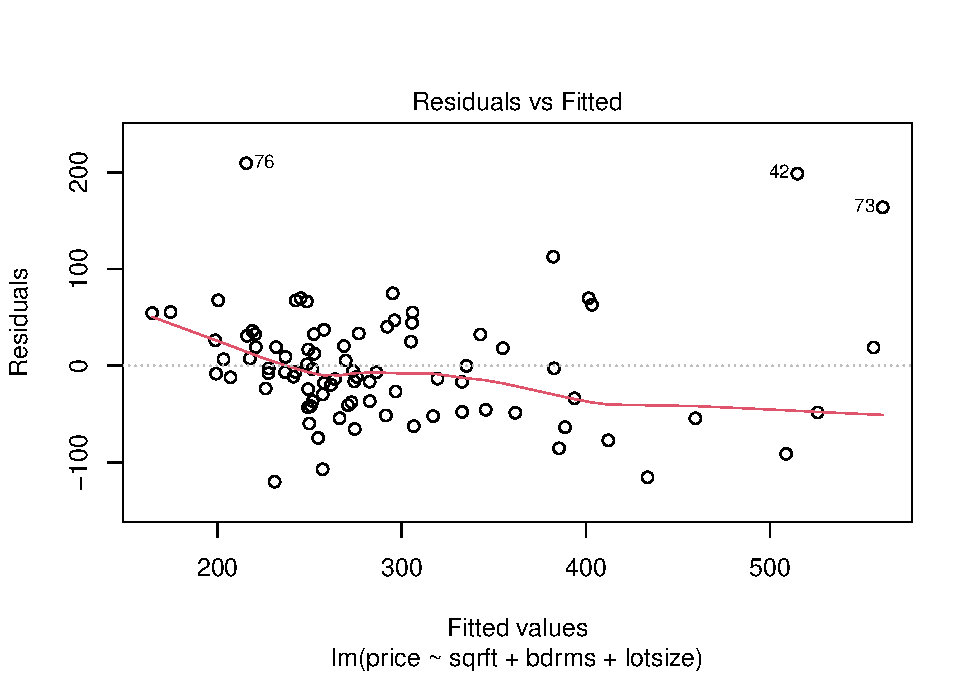
\includegraphics{Ogle_MicroMetricsAssignment_2_Q1_files/figure-latex/unnamed-chunk-15-1.pdf}

Model (d)

\begin{Shaded}
\begin{Highlighting}[]
\CommentTok{# Graphing the population model }
\KeywordTok{plot}\NormalTok{(modelD_}\DecValTok{1}\NormalTok{, }\DataTypeTok{which=}\DecValTok{1}\NormalTok{)}
\end{Highlighting}
\end{Shaded}

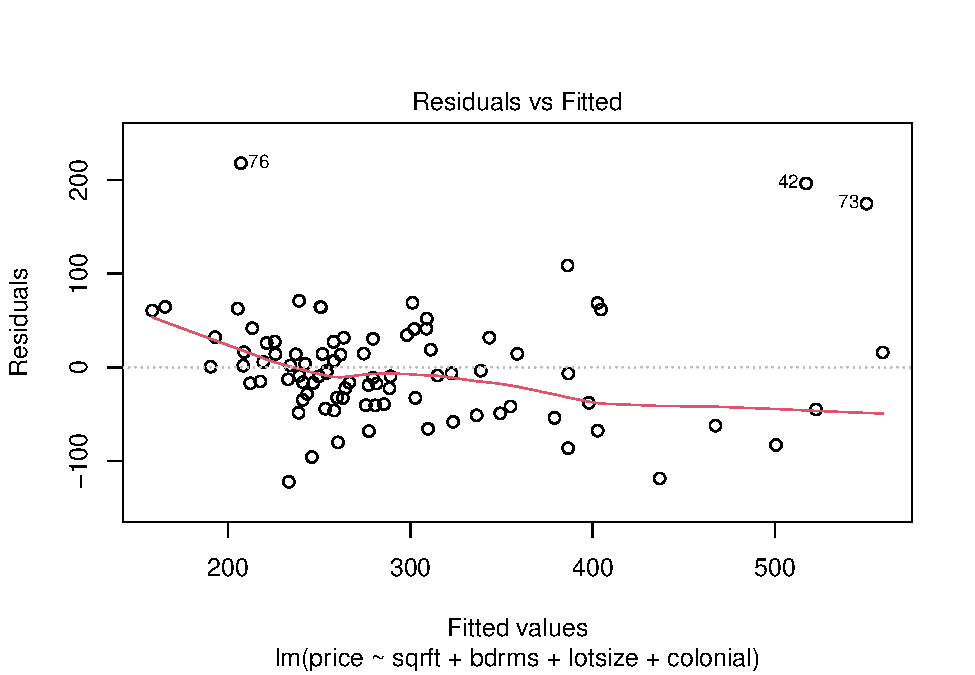
\includegraphics{Ogle_MicroMetricsAssignment_2_Q1_files/figure-latex/unnamed-chunk-16-1.pdf}

Model (f)

\begin{Shaded}
\begin{Highlighting}[]
\CommentTok{# Graphing the population model }
\KeywordTok{plot}\NormalTok{(modelF_}\DecValTok{1}\NormalTok{, }\DataTypeTok{which=}\DecValTok{1}\NormalTok{)}
\end{Highlighting}
\end{Shaded}

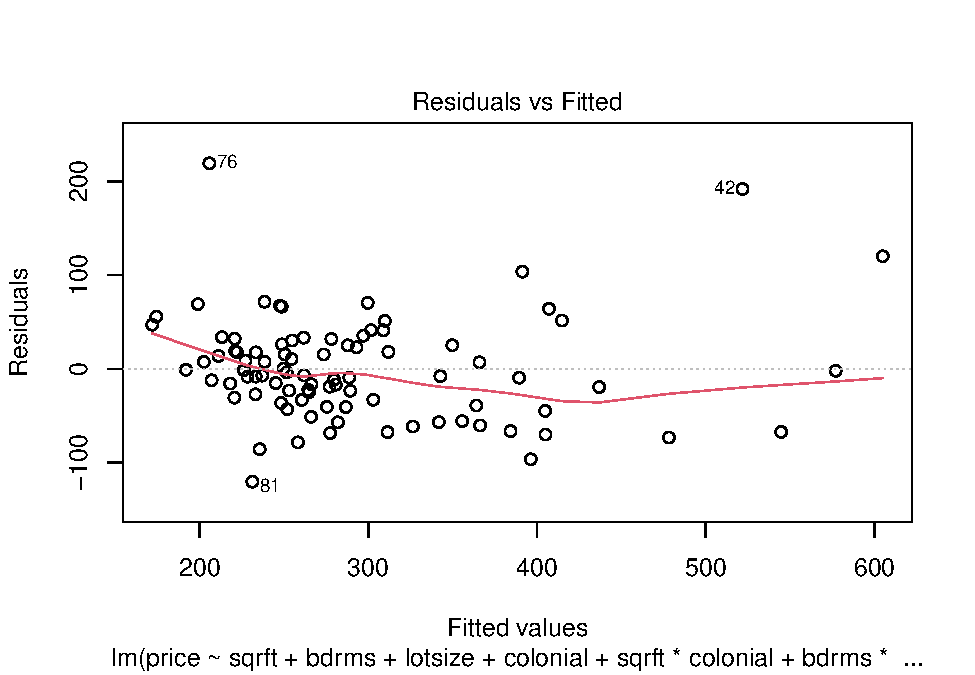
\includegraphics{Ogle_MicroMetricsAssignment_2_Q1_files/figure-latex/unnamed-chunk-17-1.pdf}

If we compare the figures above and the R-squared values for the various
models we learn two important elements about the data and the models
that we created to represent them. All the figures show strong evidence
that our models have heteroskedasticity. As we increase our fitted
values and our independent variables we see a change in the variance of
our residuals. If the models were homoskedastic the residuals would be
evenly distributed even as we increase our independent variables.

By comparing the R-squared values for (a), (d), and (f): 0.672, 0.676,
and 0.709 respectively we know that model (f) has the highest R-squared
and thus fits the data the best.

\begin{enumerate}
\def\labelenumi{(\alph{enumi})}
\setcounter{enumi}{7}
\tightlist
\item
  Heteroskedasticity means that Assumption MLR.5 of homoskedasticity is
  violated. This means that the error variance is not the same across
  all values of the independent variables. Even though under
  heteroskedasticity the estimator \(\hat\beta\) remains unbiased the
  variance of that estimator is biased and we can no longer do
  hypothesis testing. Additionally the standard errors and t-statistics
  we calculated are not correct. Additionally the standard errors are
  higher in the new model and because standard errors are related to
  variance we see a higher variance.
\end{enumerate}

We can see this through a graphic representation of the residuals v. the
fitted values and a BP test

\begin{Shaded}
\begin{Highlighting}[]
\KeywordTok{plot}\NormalTok{(modelA, }\DataTypeTok{which =} \DecValTok{1}\NormalTok{)}
\end{Highlighting}
\end{Shaded}

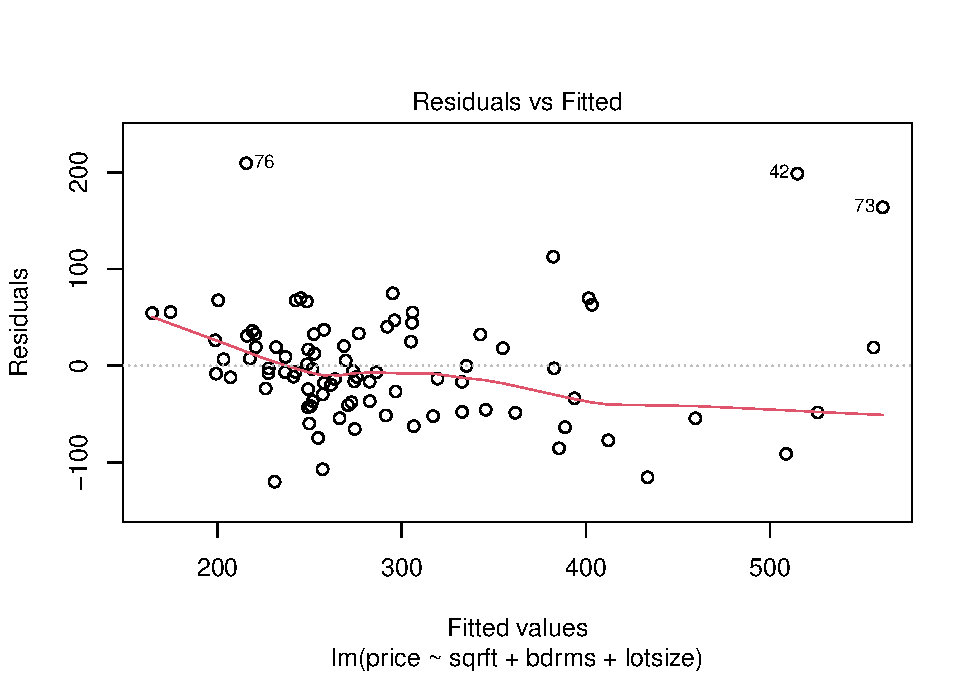
\includegraphics{Ogle_MicroMetricsAssignment_2_Q1_files/figure-latex/unnamed-chunk-18-1.pdf}

The grpahic supports our argument of heteroskedasticity because as we
increase our fitted values and our independent variables we see a change
in the variance of our residuals. If the models were homoskedastic the
residuals would be evenly distributed even as we increase our
independent variables.

Our BP value is 14.092 with three degrees of freedom and a p-value of
0.0028. This is less than our null hypothesis for homoskedasticity which
is BP value equal to 0 with statstical significance. Because we have a
p-value of less than 0.05 we reject the null and there is strong
evidence for heteroskedasticty and a violation of MLR.5.

\begin{enumerate}
\def\labelenumi{(\roman{enumi})}
\item
\end{enumerate}

\begin{table}[H] \centering 
  \caption{Regression Results (I-1)} 
  \label{} 
\begin{tabular}{@{\extracolsep{5pt}}lcc} 
\\[-1.8ex]\hline 
\hline \\[-1.8ex] 
 & \multicolumn{2}{c}{\textit{Dependent variable:}} \\ 
\cline{2-3} 
\\[-1.8ex] & \multicolumn{2}{c}{price} \\ 
 & Non-Robust Std. Errors & Robust Std. Errors \\ 
\\[-1.8ex] & (1) & (2)\\ 
\hline \\[-1.8ex] 
 sqrft & 0.123$^{***}$ & 0.123$^{***}$ \\ 
  & (0.013) & (0.018) \\ 
  & & \\ 
 bdrms & 13.853 & 13.853 \\ 
  & (9.010) & (8.479) \\ 
  & & \\ 
 lotsize & 0.002$^{***}$ & 0.002$^{***}$ \\ 
  & (0.001) & (0.001) \\ 
  & & \\ 
 Constant & $-$21.770 & $-$21.770 \\ 
  & (29.475) & (37.138) \\ 
  & & \\ 
\hline \\[-1.8ex] 
Observations & 88 & 88 \\ 
R$^{2}$ & 0.672 & 0.672 \\ 
Adjusted R$^{2}$ & 0.661 & 0.661 \\ 
Residual Std. Error (df = 84) & 59.833 & 59.833 \\ 
F Statistic (df = 3; 84) & 57.460$^{***}$ & 23.72$^{***}$ \\ 
\hline 
\hline \\[-1.8ex] 
\textit{Note:}  & \multicolumn{2}{r}{$^{*}$p$<$0.1; $^{**}$p$<$0.05; $^{***}$p$<$0.01} \\ 
 & \multicolumn{2}{r}{Standard errors in parentheses} \\ 
\end{tabular} 
\end{table}

For square footage and lot size coefficients the robust standard errors
are larger than the non-robust standard errors. We see a decrease in the
robust standard error for the bedroom coefficient, however, this result
is not statistically significant. We already know that there is
heteroskedasticity present in the model. We use robust standard errors
to correct for the heteroskedascity in the model. Therefore our results
from a remain the same however, because the standard error increases we
have understand that the average distance that the observed values fall
from the regression line increases.

\begin{enumerate}
\def\labelenumi{(\alph{enumi})}
\setcounter{enumi}{9}
\item
\end{enumerate}

\begin{enumerate}
\def\labelenumi{\roman{enumi})}
\tightlist
\item
  We estimate the population model: \[
  lprice_i = \beta_0 + \beta_1sqrft_i + \beta_2bdrms_i + \beta_3lotsize_i + U_i
  \]

  \begin{table}[H] \centering 
    \caption{Regression Results (j-1)} 
    \label{} 
  \begin{tabular}{@{\extracolsep{5pt}}lc} 
  \\[-1.8ex]\hline 
  \hline \\[-1.8ex] 
   & \multicolumn{1}{c}{\textit{Dependent variable:}} \\ 
  \cline{2-2} 
  \\[-1.8ex] & lprice \\ 
  \hline \\[-1.8ex] 
   sqrft & 0.0004$^{***}$ \\ 
    & (0.00004) \\ 
    & \\ 
   bdrms & 0.025 \\ 
    & (0.029) \\ 
    & \\ 
   lotsize & 0.00001$^{***}$ \\ 
    & (0.00000) \\ 
    & \\ 
   Constant & 4.759$^{***}$ \\ 
    & (0.094) \\ 
    & \\ 
  \hline \\[-1.8ex] 
  Observations & 88 \\ 
  R$^{2}$ & 0.622 \\ 
  Adjusted R$^{2}$ & 0.609 \\ 
  Residual Std. Error & 0.190 (df = 84) \\ 
  F Statistic & 46.128$^{***}$ (df = 3; 84) \\ 
  \hline 
  \hline \\[-1.8ex] 
  \textit{Note:}  & \multicolumn{1}{r}{$^{*}$p$<$0.1; $^{**}$p$<$0.05; $^{***}$p$<$0.01} \\ 
   & \multicolumn{1}{r}{Standard errors in parentheses} \\ 
  \end{tabular} 
  \end{table}
\item
  According to our regression results from the table above we can
  interpret the following.
\end{enumerate}

All other independent variables constant for every unit increase in
square footage the house price in dollars increases 0.04\% on average.

All other independent variables constant for every unit increase in
bedrooms the house price in dollars increases 2.5\% on average.

All other independent variables constant for every unit increase in lot
size the house price in dollars increases 0.001\% on average.

When there are no effects from any independent variables, when they are
all equal to zero the average price is 4,759. However, this value is not
statistically significant in this regression because the p value is
greater than 0.05.

\begin{enumerate}
\def\labelenumi{(\alph{enumi})}
\setcounter{enumi}{10}
\tightlist
\item
  Heteroskedasticity means that Assumption MLR.5 of homoskedasticity is
  violated. This means that the error variance is not the same across
  all values of the independent variables. Even though under
  heteroskedasticity the estimator \(\hat\beta\) remains unbiased the
  variance of that estimator is biased and we can no longer do
  hypothesis testing. Additionally the standard errors and t-statistics
  we calculated are not correct. Additionally the standard errors are
  higher in the new model and because standard errors are related to
  variance we see a higher variance.
\end{enumerate}

We can see this through a graphic representation of the residuals v. the
fitted values and a BP test

\begin{Shaded}
\begin{Highlighting}[]
\KeywordTok{plot}\NormalTok{(modelJ_}\DecValTok{1}\NormalTok{, }\DataTypeTok{which =} \DecValTok{1}\NormalTok{)}
\end{Highlighting}
\end{Shaded}

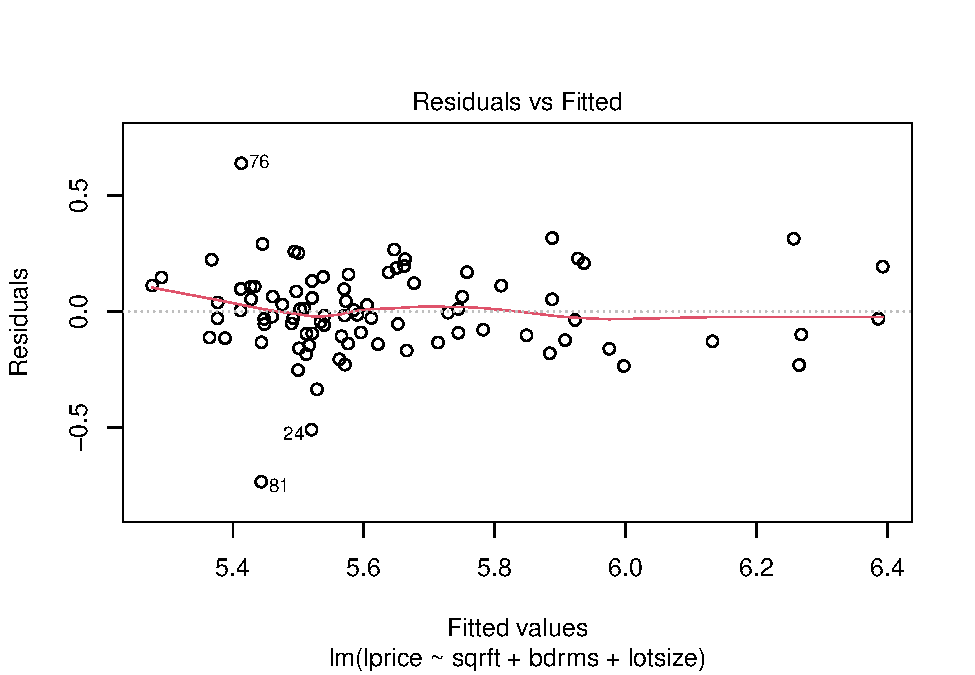
\includegraphics{Ogle_MicroMetricsAssignment_2_Q1_files/figure-latex/unnamed-chunk-22-1.pdf}

The graphic supports our argument of homooskedasticity because as we
increase our fitted values and our independent variables we do not see a
change in the variance of our residuals. The model is homoskedastic
because the residuals are evenly distributed even as we increase our
independent variables.

Our BP value is 3.543 with three degrees of freedom and a p-value of
0.315. Our null hypothesis is that if our BP value is equal to 0 than
there is homoskedasticity in the model. Because we have a p-value of
greater than 0.05 we fail to reject the null and there is strong
evidence for homoskedacitiy and MLR.5 is held. Our boss is right using
log price instead of price fixes our model and makes it homoskedastic.

\begin{enumerate}
\def\labelenumi{(\alph{enumi})}
\setcounter{enumi}{11}
\tightlist
\item
  To see if we should include sqrft in the model we need to calculate
  the OVB for the estimator for bedrooms.
\end{enumerate}

\begin{table}[!htbp] \centering 
  \caption{Regression Results (l-1)} 
  \label{} 
\begin{tabular}{@{\extracolsep{5pt}}lcc} 
\\[-1.8ex]\hline 
\hline \\[-1.8ex] 
 & \multicolumn{2}{c}{\textit{Dependent variable:}} \\ 
\cline{2-3} 
\\[-1.8ex] & \multicolumn{2}{c}{price} \\ 
\\[-1.8ex] & (1) & (2)\\ 
\hline \\[-1.8ex] 
 sqrft & 0.123$^{***}$ &  \\ 
  & (0.013) &  \\ 
  & & \\ 
 bdrms & 13.853 & 57.313$^{***}$ \\ 
  & (9.010) & (10.885) \\ 
  & & \\ 
 lotsize & 0.002$^{***}$ & 0.003$^{***}$ \\ 
  & (0.001) & (0.001) \\ 
  & & \\ 
 Constant & $-$21.770 & 63.262 \\ 
  & (29.475) & (39.620) \\ 
  & & \\ 
\hline \\[-1.8ex] 
Observations & 88 & 88 \\ 
R$^{2}$ & 0.672 & 0.337 \\ 
Adjusted R$^{2}$ & 0.661 & 0.321 \\ 
Residual Std. Error & 59.833 (df = 84) & 84.624 (df = 85) \\ 
F Statistic & 57.460$^{***}$ (df = 3; 84) & 21.585$^{***}$ (df = 2; 85) \\ 
\hline 
\hline \\[-1.8ex] 
\textit{Note:}  & \multicolumn{2}{r}{$^{*}$p$<$0.1; $^{**}$p$<$0.05; $^{***}$p$<$0.01} \\ 
 & \multicolumn{2}{r}{Standard errors in parentheses} \\ 
\end{tabular} 
\end{table}

We can see that the coefficient for bedrooms increase from 12.853 to
57.313. Thus the OVB for this coefficient is -44.46. Omitting sqrft
increases the bedrooms effect on price. And it increases the variance of
that effect on price as we see an increase in the standard error.
Standard error is a statistic that is correlated with variance. And
variance increases. Yes we should included sqrft because we want to
minimize variance and the adjusted r-squared value increases.

Problem 3 (a) The causal question is related to proving the Solow Growth
Model through modern data about GDP and GDP growth taken from 1960-2021.
Specifically, we want to study if real income is higher in countries
with higher savings rates and lower in countries with higher values of
\({ n + g + \delta}\). We want to see how log(I/GDP) and
log(\({ n + g + \delta}\)) (X) effect log(GDP) per working age person in
2021 (Y). We assume that g + delta are constant over every country and
equal to 0.05.

\begin{enumerate}
\def\labelenumi{(\alph{enumi})}
\setcounter{enumi}{1}
\item
  The ideal experiment would need a large random sample of countries all
  with the exact same economies and we could measure how Investment /
  GDP and n the average rate of growth of the working age population
  (age defined as 14 to 64) on the log gdp of a working age person in
  2021.
\item
  Some issues with the ideal experiment are that cannot just clone
  countries economies, population, and size. Countries are huge entities
  which have complex and intricate differences that cannot be
  duplicated.
\item
  I might add controls like measures for Human capital to control the
  variability among countries. An example might be the varying levels of
  education. This would increase the credibility of MLR.4 being true
  because educational achievement is correlated to investment and GDP an
  independent variable. Thus if we include it, remove it from our error
  term it will make the Zero Conditional Mean assumption more credible
  and make the assumption that our estimator is unbiased.
\end{enumerate}

\end{document}
